%  LaTeX support: latex@mdpi.com 
%  For support, please attach all files needed for compiling as well as the log file, and specify your operating system, LaTeX version, and LaTeX editor.

%=================================================================
\documentclass[journal,article,submit,pdftex,moreauthors]{Definitions/mdpi} 

%--------------------
% Class Options:
%--------------------
%----------
% journal
%----------
% Choose between the following MDPI journals:
% acoustics, actuators, addictions, admsci, adolescents, aerobiology, aerospace, agriculture, agriengineering, agrochemicals, agronomy, ai, air, algorithms, allergies, alloys, analytica, analytics, anatomia, animals, antibiotics, antibodies, antioxidants, applbiosci, appliedchem, appliedmath, applmech, applmicrobiol, applnano, applsci, aquacj, architecture, arm, arthropoda, arts, asc, asi, astronomy, atmosphere, atoms, audiolres, automation, axioms, bacteria, batteries, bdcc, behavsci, beverages, biochem, bioengineering, biologics, biology, biomass, biomechanics, biomed, biomedicines, biomedinformatics, biomimetics, biomolecules, biophysica, biosensors, biotech, birds, bloods, blsf, brainsci, breath, buildings, businesses, cancers, carbon, cardiogenetics, catalysts, cells, ceramics, challenges, chemengineering, chemistry, chemosensors, chemproc, children, chips, cimb, civileng, cleantechnol, climate, clinpract, clockssleep, cmd, coasts, coatings, colloids, colorants, commodities, compounds, computation, computers, condensedmatter, conservation, constrmater, cosmetics, covid, crops, cryptography, crystals, csmf, ctn, curroncol, cyber, dairy, data, ddc, dentistry, dermato, dermatopathology, designs, devices, diabetology, diagnostics, dietetics, digital, disabilities, diseases, diversity, dna, drones, dynamics, earth, ebj, ecologies, econometrics, economies, education, ejihpe, electricity, electrochem, electronicmat, electronics, encyclopedia, endocrines, energies, eng, engproc, entomology, entropy, environments, environsciproc, epidemiologia, epigenomes, est, fermentation, fibers, fintech, fire, fishes, fluids, foods, forecasting, forensicsci, forests, foundations, fractalfract, fuels, future, futureinternet, futurepharmacol, futurephys, futuretransp, galaxies, games, gases, gastroent, gastrointestdisord, gels, genealogy, genes, geographies, geohazards, geomatics, geosciences, geotechnics, geriatrics, grasses, gucdd, hazardousmatters, healthcare, hearts, hemato, hematolrep, heritage, higheredu, highthroughput, histories, horticulturae, hospitals, humanities, humans, hydrobiology, hydrogen, hydrology, hygiene, idr, ijerph, ijfs, ijgi, ijms, ijns, ijpb, ijtm, ijtpp, ime, immuno, informatics, information, infrastructures, inorganics, insects, instruments, inventions, iot, j, jal, jcdd, jcm, jcp, jcs, jcto, jdb, jeta, jfb, jfmk, jimaging, jintelligence, jlpea, jmmp, jmp, jmse, jne, jnt, jof, joitmc, jor, journalmedia, jox, jpm, jrfm, jsan, jtaer, jvd, jzbg, kidneydial, kinasesphosphatases, knowledge, land, languages, laws, life, liquids, literature, livers, logics, logistics, lubricants, lymphatics, machines, macromol, magnetism, magnetochemistry, make, marinedrugs, materials, materproc, mathematics, mca, measurements, medicina, medicines, medsci, membranes, merits, metabolites, metals, meteorology, methane, metrology, micro, microarrays, microbiolres, micromachines, microorganisms, microplastics, minerals, mining, modelling, molbank, molecules, mps, msf, mti, muscles, nanoenergyadv, nanomanufacturing,\gdef\@continuouspages{yes}} nanomaterials, ncrna, ndt, network, neuroglia, neurolint, neurosci, nitrogen, notspecified, %%nri, nursrep, nutraceuticals, nutrients, obesities, oceans, ohbm, onco, %oncopathology, optics, oral, organics, organoids, osteology, oxygen, parasites, parasitologia, particles, pathogens, pathophysiology, pediatrrep, pharmaceuticals, pharmaceutics, pharmacoepidemiology,\gdef\@ISSN{2813-0618}\gdef\@continuous pharmacy, philosophies, photochem, photonics, phycology, physchem, physics, physiologia, plants, plasma, platforms, pollutants, polymers, polysaccharides, poultry, powders, preprints, proceedings, processes, prosthesis, proteomes, psf, psych, psychiatryint, psychoactives, publications, quantumrep, quaternary, qubs, radiation, reactions, receptors, recycling, regeneration, religions, remotesensing, reports, reprodmed, resources, rheumato, risks, robotics, ruminants, safety, sci, scipharm, sclerosis, seeds, sensors, separations, sexes, signals, sinusitis, skins, smartcities, sna, societies, socsci, software, soilsystems, solar, solids, spectroscj, sports, standards, stats, std, stresses, surfaces, surgeries, suschem, sustainability, symmetry, synbio, systems, targets, taxonomy, technologies, telecom, test, textiles, thalassrep, thermo, tomography, tourismhosp, toxics, toxins, transplantology, transportation, traumacare, traumas, tropicalmed, universe, urbansci, uro, vaccines, vehicles, venereology, vetsci, vibration, virtualworlds, viruses, vision, waste, water, wem, wevj, wind, women, world, youth, zoonoticdis 
% For posting an early version of this manuscript as a preprint, you may use "preprints" as the journal. Changing "submit" to "accept" before posting will remove line numbers.

%---------
% article
%---------
% The default type of manuscript is "article", but can be replaced by: 
% abstract, addendum, article, book, bookreview, briefreport, casereport, comment, commentary, communication, conferenceproceedings, correction, conferencereport, entry, expressionofconcern, extendedabstract, datadescriptor, editorial, essay, erratum, hypothesis, interestingimage, obituary, opinion, projectreport, reply, retraction, review, perspective, protocol, shortnote, studyprotocol, systematicreview, supfile, technicalnote, viewpoint, guidelines, registeredreport, tutorial
% supfile = supplementary materials

%----------
% submit
%----------
% The class option "submit" will be changed to "accept" by the Editorial Office when the paper is accepted. This will only make changes to the frontpage (e.g., the logo of the journal will get visible), the headings, and the copyright information. Also, line numbering will be removed. Journal info and pagination for accepted papers will also be assigned by the Editorial Office.

%------------------
% moreauthors
%------------------
% If there is only one author the class option oneauthor should be used. Otherwise use the class option moreauthors.

%---------
% pdftex
%---------
% The option pdftex is for use with pdfLaTeX. Remove "pdftex" for (1) compiling with LaTeX & dvi2pdf (if eps figures are used) or for (2) compiling with XeLaTeX.

%=================================================================
% MDPI internal commands - do not modify
\firstpage{1} 
\makeatletter 
\setcounter{page}{\@firstpage} 
\makeatother
\pubvolume{1}
\issuenum{1}
\articlenumber{0}
\pubyear{2023}
\copyrightyear{2023}
%\externaleditor{Academic Editor: Firstname Lastname}
\datereceived{ } 
\daterevised{ } % Comment out if no revised date
\dateaccepted{ } 
\datepublished{ } 
%\datecorrected{} % For corrected papers: "Corrected: XXX" date in the original paper.
%\dateretracted{} % For corrected papers: "Retracted: XXX" date in the original paper.
\hreflink{https://doi.org/} % If needed use \linebreak
%\doinum{}
%\pdfoutput=1 % Uncommented for upload to arXiv.org

%=================================================================
% Add packages and commands here. The following packages are loaded in our class file: fontenc, inputenc, calc, indentfirst, fancyhdr, graphicx, epstopdf, lastpage, ifthen, float, amsmath, amssymb, lineno, setspace, enumitem, mathpazo, booktabs, titlesec, etoolbox, tabto, xcolor, colortbl, soul, multirow, microtype, tikz, totcount, changepage, attrib, upgreek, array, tabularx, pbox, ragged2e, tocloft, marginnote, marginfix, enotez, amsthm, natbib, hyperref, cleveref, scrextend, url, geometry, newfloat, caption, draftwatermark, seqsplit
% cleveref: load \crefname definitions after \begin{document}

%=================================================================
% Please use the following mathematics environments: Theorem, Lemma, Corollary, Proposition, Characterization, Property, Problem, Example, ExamplesandDefinitions, Hypothesis, Remark, Definition, Notation, Assumption
%% For proofs, please use the proof environment (the amsthm package is loaded by the MDPI class).

%=================================================================
% Full title of the paper (Capitalized)
\Title{Unsupervised learning in in shallow marine environments using satellite imagery}

% MDPI internal command: Title for citation in the left column
\TitleCitation{Title}

% Author Orchid ID: enter ID or remove command
\newcommand{\orcidauthorA}{0000-0000-0000-000X} % Add \orcidA{} behind the author's name
%\newcommand{\orcidauthorB}{0000-0000-0000-000X} % Add \orcidB{} behind the author's name

% Authors, for the paper (add full first names)
\Author{Zayad AlZayer$^{1,\dagger,\ddagger}$\orcidA{}, Cedric John$^{2,\ddagger}$ and Philippa Mason$^{2,}$*}

%\longauthorlist{yes}

% MDPI internal command: Authors, for metadata in PDF
\AuthorNames{Zayan AlZayer, Philippa Mason and Cedric John}

% MDPI internal command: Authors, for citation in the left column
\AuthorCitation{AlZayer, Z.; Mason, P.; John, C.}
% If this is a Chicago style journal: Lastname, Firstname, Firstname Lastname, and Firstname Lastname.

% Affiliations / Addresses (Add [1] after \address if there is only one affiliation.)
\address{%
$^{1}$ \quad Imperial College 1; zba21@ic.ac.uk\\
$^{2}$ \quad Affiliation 2; e-mail@e-mail.com}

% Contact information of the corresponding author
\corres{Correspondence: e-mail@e-mail.com; Tel.: (optional; include country code; if there are multiple corresponding authors, add author initials) +xx-xxxx-xxx-xxxx (F.L.)}

% Current address and/or shared authorship
\firstnote{Current address: Affiliation 3.} 
\secondnote{These authors contributed equally to this work.}
% The commands \thirdnote{} till \eighthnote{} are available for further notes

%\simplesumm{} % Simple summary

%\conference{} % An extended version of a conference paper

% Abstract (Do not insert blank lines, i.e. \\) 
\abstract{This paper presents an approach to habitat mappiong using multispectral sentinel-2 data. This approach is based on using 8 indices, Principal component analysis, Uniform manifold approximation projection (UMAP), K-means clustering and XGboost. This multi-faceted 
approach allows us to effectively analyse and interpret multispectral data. The results show that the approach is able to identify and classify different habitats in shallow marine environments.}

% Keywords
\keyword{Shallow Water; Remote sensing; Machine learning; Coral Reefs} 

% The fields PACS, MSC, and JEL may be left empty or commented out if not applicable
%\PACS{J0101}
%\MSC{}
%\JEL{}

%%%%%%%%%%%%%%%%%%%%%%%%%%%%%%%%%%%%%%%%%%
% Only for the journal Diversity
%\LSID{\url{http://}}

%%%%%%%%%%%%%%%%%%%%%%%%%%%%%%%%%%%%%%%%%%
% Only for the journal Applied Sciences
%\featuredapplication{Authors are encouraged to provide a concise description of the specific application or a potential application of the work. This section is not mandatory.}
%%%%%%%%%%%%%%%%%%%%%%%%%%%%%%%%%%%%%%%%%%

%%%%%%%%%%%%%%%%%%%%%%%%%%%%%%%%%%%%%%%%%%
% Only for the journal Data
%\dataset{DOI number or link to the deposited data set if the data set is published separately. If the data set shall be published as a supplement to this paper, this field will be filled by the journal editors. In this case, please submit the data set as a supplement.}
%\datasetlicense{License under which the data set is made available (CC0, CC-BY, CC-BY-SA, CC-BY-NC, etc.)}

%%%%%%%%%%%%%%%%%%%%%%%%%%%%%%%%%%%%%%%%%%
% Only for the journal Toxins
%\keycontribution{The breakthroughs or highlights of the manuscript. Authors can write one or two sentences to describe the most important part of the paper.}

%%%%%%%%%%%%%%%%%%%%%%%%%%%%%%%%%%%%%%%%%%
% Only for the journal Encyclopedia
%\encyclopediadef{For entry manuscripts only: please provide a brief overview of the entry title instead of an abstract.}

%%%%%%%%%%%%%%%%%%%%%%%%%%%%%%%%%%%%%%%%%%
% Only for the journal Advances in Respiratory Medicine
%\addhighlights{yes}
%\renewcommand{\addhighlights}{%

%\noindent This is an obligatory section in “Advances in Respiratory Medicine”, whose goal is to increase the discoverability and readability of the article via search engines and other scholars. Highlights should not be a copy of the abstract, but a simple text allowing the reader to quickly and simplified find out what the article is about and what can be cited from it. Each of these parts should be devoted up to 2~bullet points.\vspace{3pt}\\
%\textbf{What are the main findings?}
% \begin{itemize}[labelsep=2.5mm,topsep=-3pt]
% \item First bullet.
% \item Second bullet.
% \end{itemize}\vspace{3pt}
%\textbf{What is the implication of the main finding?}
% \begin{itemize}[labelsep=2.5mm,topsep=-3pt]
% \item First bullet.
% \item Second bullet.
% \end{itemize}
%}
\usepackage{natbib}
%%%%%%%%%%%%%%%%%%%%%%%%%%%%%%%%%%%%%%%%%%
\begin{document}

%%%%%%%%%%%%%%%%%%%%%%%%%%%%%%%%%%%%%%%%%%

\section{Introduction}

Over the past 40 years, the crucial yet challenging task of monitoring coral reefs has been undertaken, with data gathering initiatives tracing back to as early as the 1960s \cite{goreau1964mass}, and more comprehensive databases from the 1980s to 2022 \cite{Woesik2022},  as well as
citizen science datasets \cite{ALA2021}.With these data sets encompassing sub-mapping scale information, remote sensing studies encompass a broad range of objectives, from local ecological surveillance to tracking carbon budgets \cite{duarte2017reviews}. In light of the threats imposed 
by climate change and anthropogenic activities \cite{hughes2010rising}, 
and the rapid temperature rise that has led to a reduction in both coral cover and diversity \cite{bruno2007thermal} \cite{pandolfi2003global} \cite{hoegh2007coral}, there exists an immediate and pressing need for accurate and swift global coral reef monitoring and data fusion techniques.


Much research has centered around supervised learning algorithms \cite{su14106161} \cite{white2021coral} \cite{pavoni2022taglab} \cite{zeng2022spectral}, with supervised learning generally more commonly applied on Sentinel-2 data \cite{phiri2020sentinel}. 
Supervised learning, a form of machine learning that utilizes labeled data to train a model, thereby enabling it to predict labels for new data.
This has been applied at a variety of scales from classification of individual corals to entire satellite images. However, this approach often entails certain assumptions about the labeled data, including a uniform quality of labels among all labelers \cite{sheng2008get}, 
thereby necessitating expert verification. This methodology has been applied to categorize images of coral reefs into various classes such as coral, sand, algae, and rubble \cite{Li2020}. 
Nevertheless, such a process requires labeled data, which can be challenging to procure and process. Moreover, it can be outright impossible in cases dealing with historical satellite imagery, where the ground truth may not always be accessible in an environment that is living and adapting.

Atmospheric corrections are also necessary for optical imaging 


()\cite{louis2016sentinel} reflectance uncertainty up to 0.06 for NDVI), using the sen2cor atmospheric processor, it uses a combination of DDV (Dark Dense Vegetation) pixels to apply an atmospheric correction based on the \cite{atmospheric_correction1988}

Unsupervised learning uses unlabelled data to train a model to find patterns in the data itself, helping unlock bottlenecks that exist within labelled data \cite{usama2019unsupervised}.

In this study we aim to use a combination of unsupervised and supervised learning to classify coral reefs into different classes. Using a combination of more traditional clustering methods and various color spaces. 
We then use a supervised learning algorithms to provide additional insight into the clustering and 
retrieve understandable results from the data and its clusters, including using simple logistic regression to gain insight into the data itself.

\citep{Hedley2016} provide a comprehensive overview of sensor limitations and uses for coral reef monitoring, including the use of satellite imagery. Many challenges exist in the processing of the data, one such problem is 
sea roughness due to wind is also a problem as very large changes in reflectance such as sun glint also affect the imagery negatively  and should generally be discarded and or masked out \cite{gordon1997atmospheric}

Object based segmentation methods have had good success at discriminating classes of various corals \cite{Nguyen2021}, with studies combining both pixel based methods and object based methods 
also showing a high degree of accuracy in water bodies \cite{huang2015combining}.


\cite{zekoll2021comparison} Provide a comprehensive comparison of three masking algorithms, fmask, Sen2Cor and ATCOR, with f-mask producing the highest class accuracy for water bodies and Sen2Cor 
highest overall accuracy for water scenes. F-mask also produces the highest overall accuracy for cloudy scenes. This is relevant to the discussion as these have been used as intermediate steps in the processing of the data.
and understanding overall sources of error and uncertainty in the data is important for understanding the results of the clustering and classification. Comparisons of the algorithms versus supervised machine learning approaches have been
done by \cite{raiyani2021sentinel}, with results indicating that machine learning approaches outperforming the Sen2Cor scene classification.



%%%%%%%%%%%%%%%%%%%%%%%%%%%%%%%%%%%%%%%%%%
\section{Methods}
In this study we setup a series of systematic experiments using the workflow described briefly below. 

\begin{figure}
	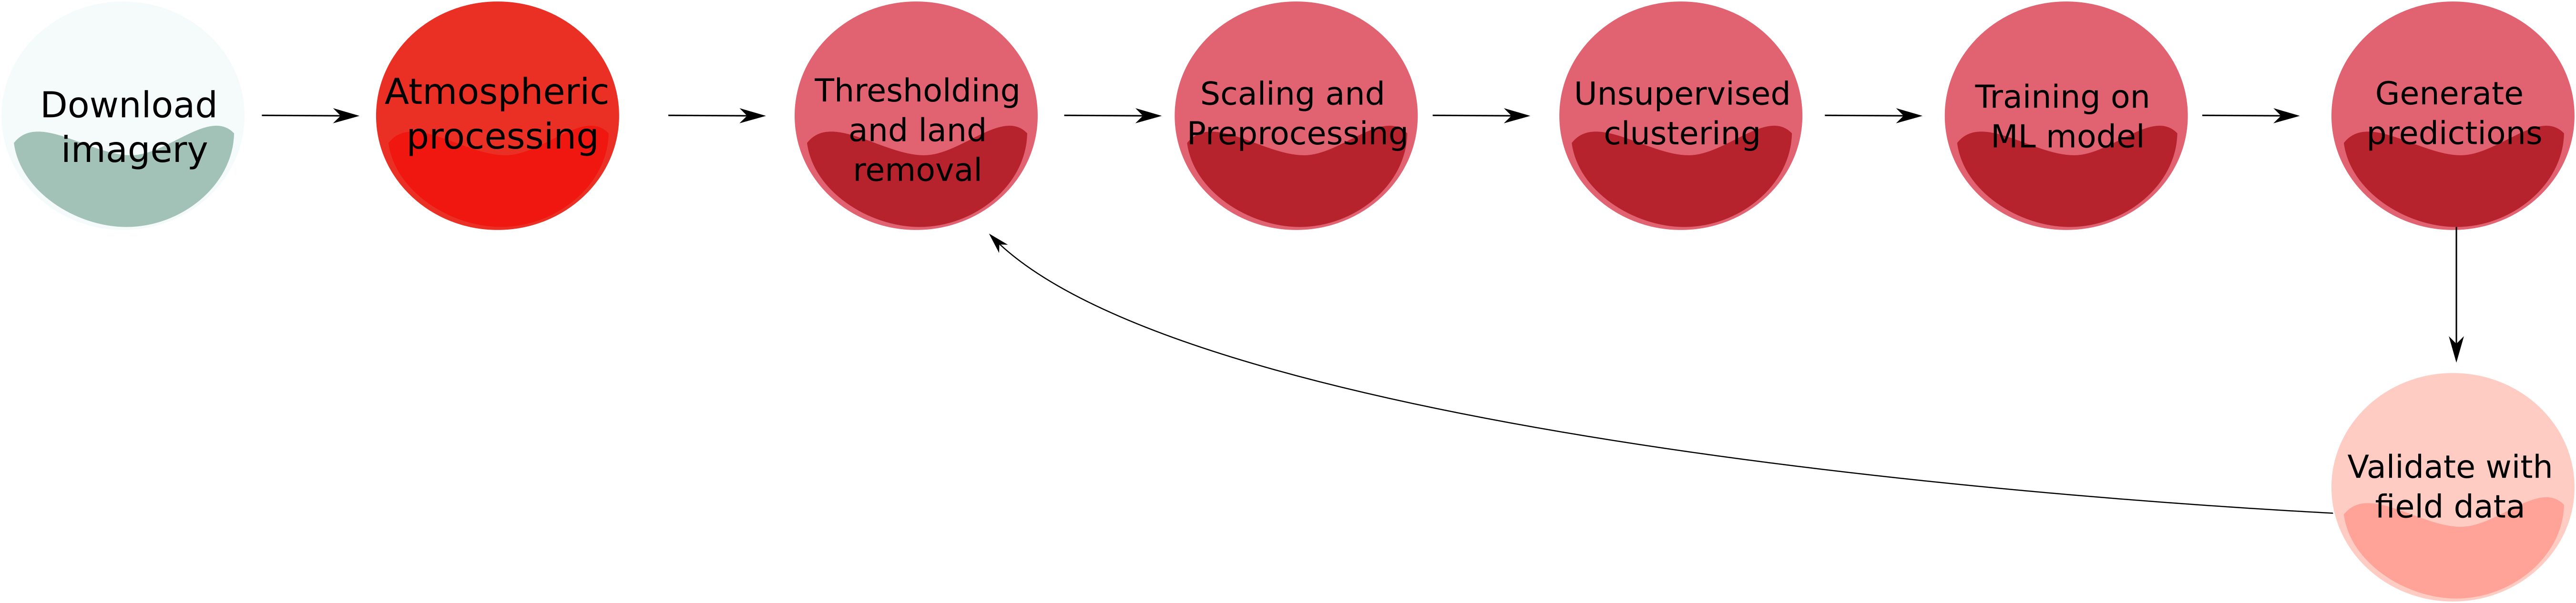
\includegraphics[width=\linewidth]{Images/Flow_Chart.png}
	\caption{Basic overall workflow in the study of coral reefs using Sentinel-2 imagery}
	\label{fig:workflow}
\end{figure}

\begin{figure}
	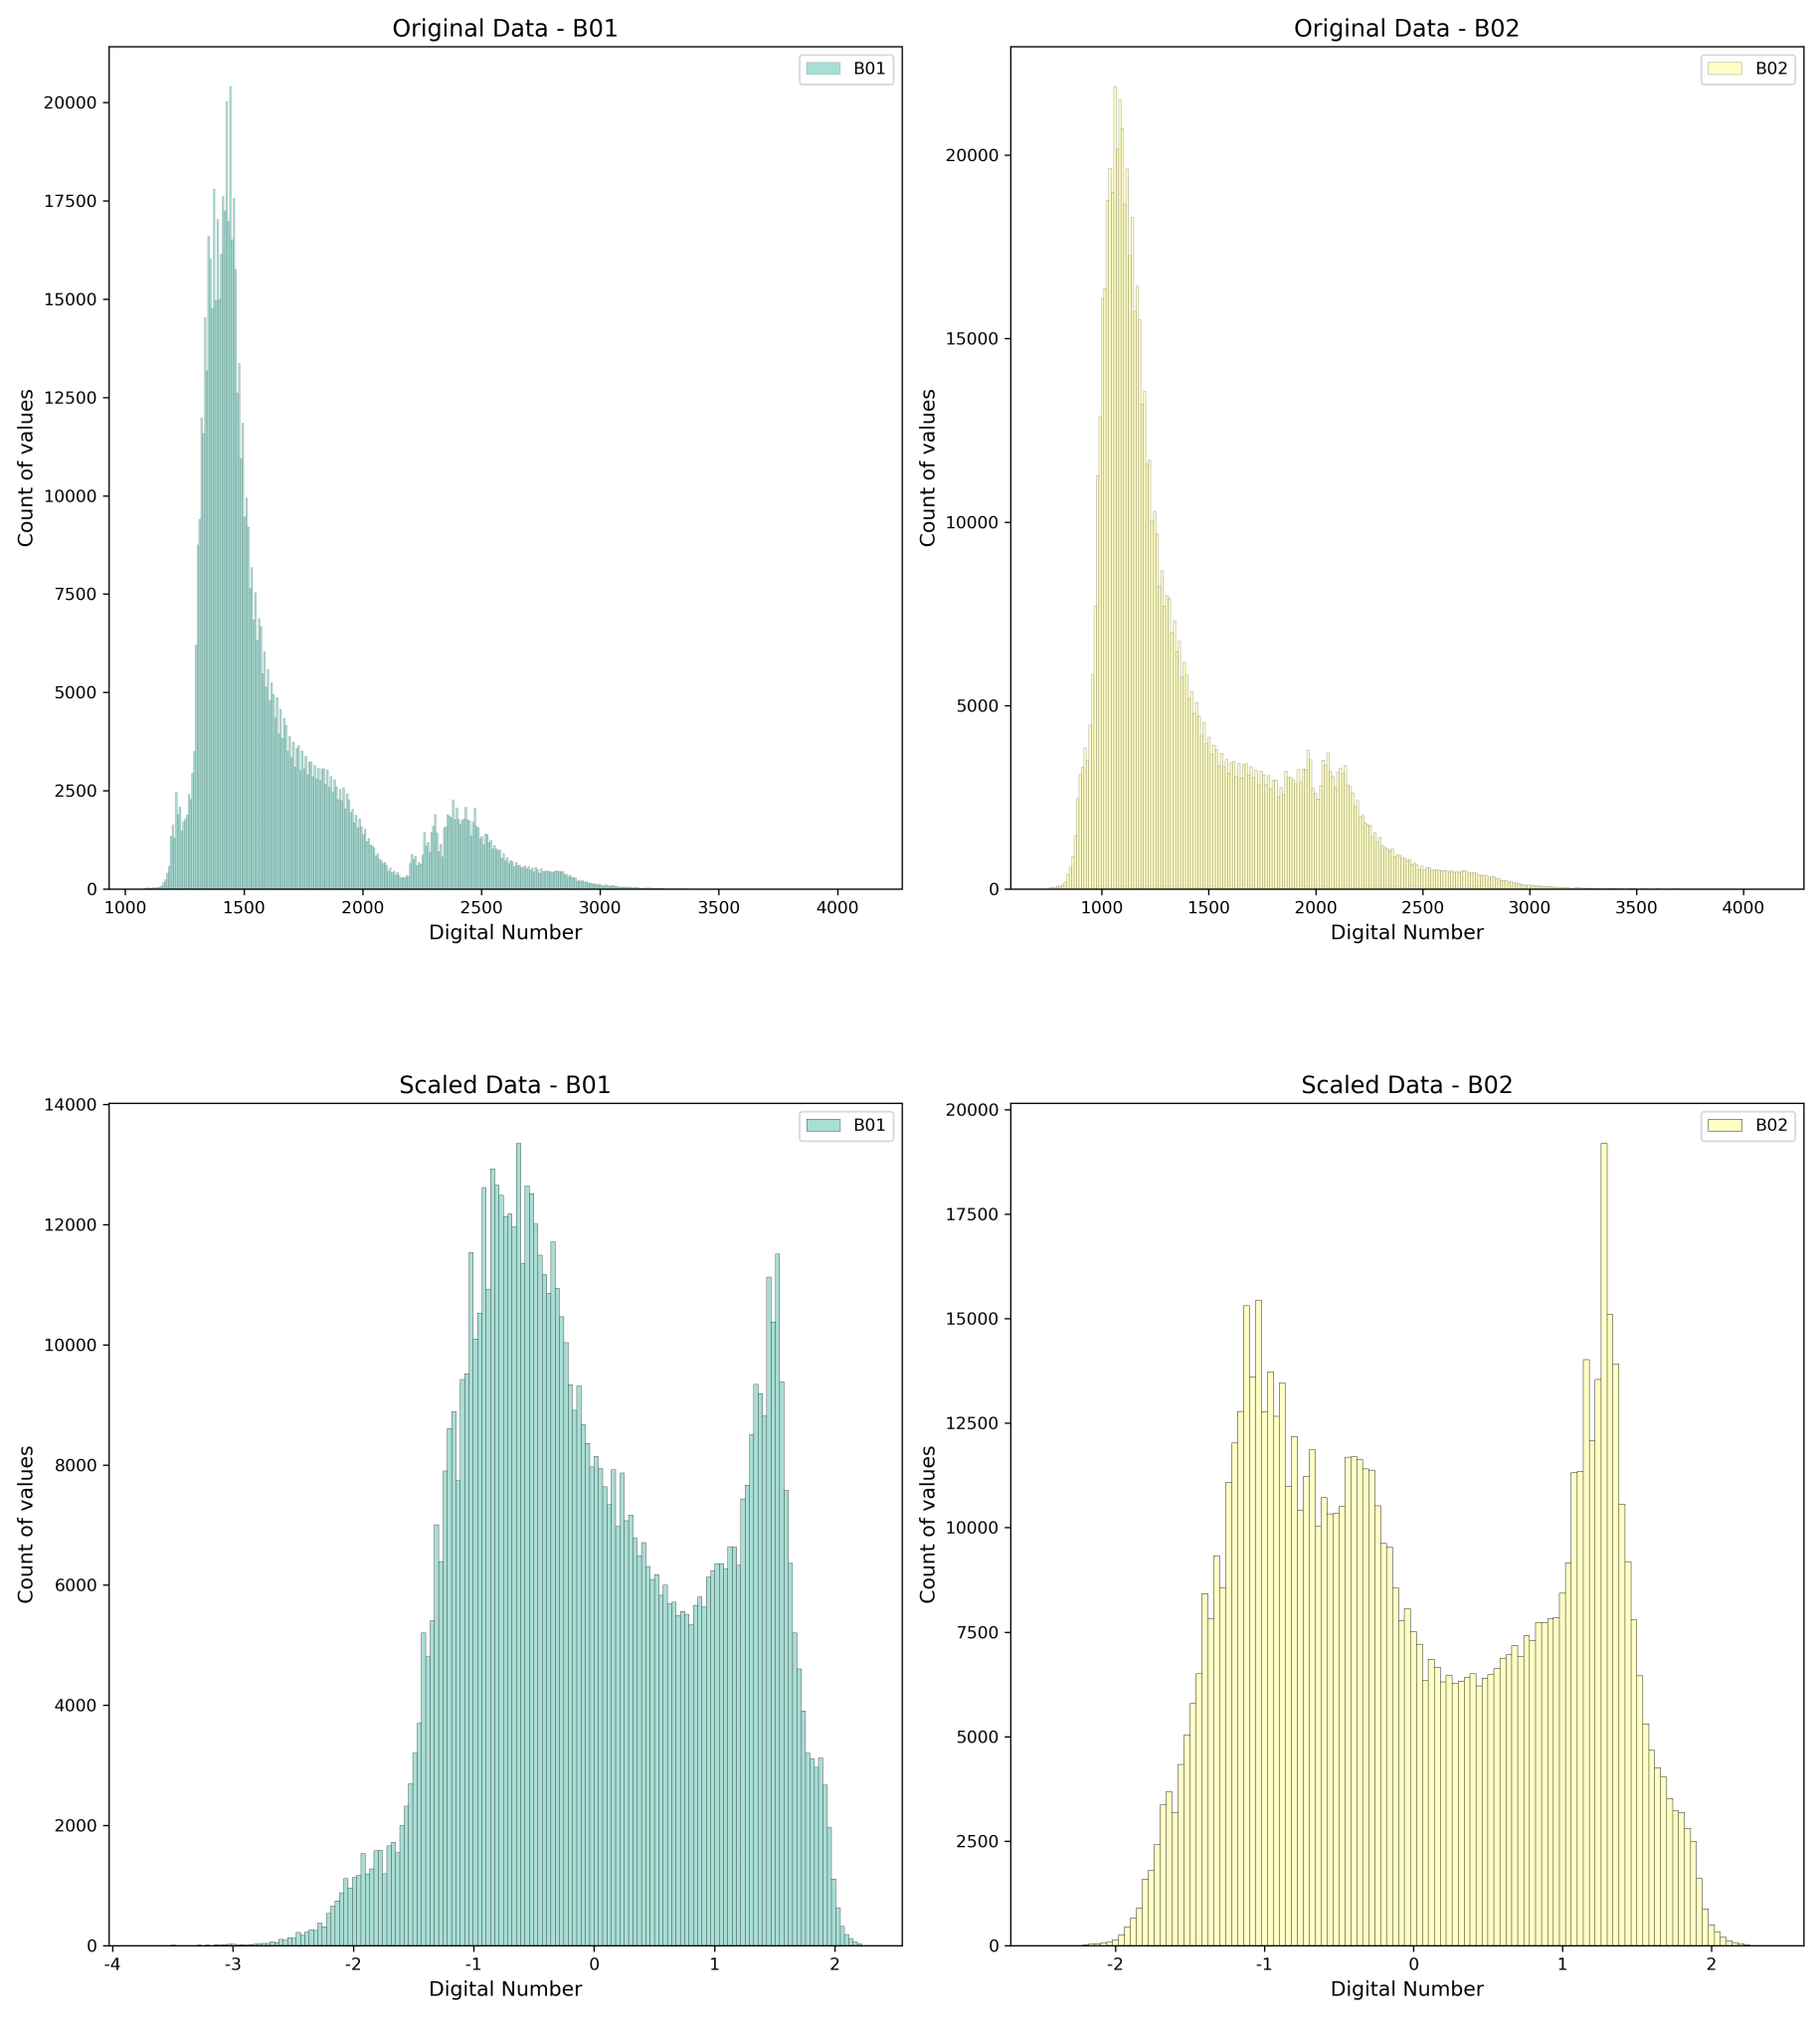
\includegraphics[width=\linewidth]{Images/Scaling_Training_Data.png}
	\caption{Data transformations applied to the training dataset}
	\label{fig:Scaling}
\end{figure}

\begin{itemize}
	\item Data collection and preprocessing: We gather Sentinel-2 L1C data using the API provided by the Copernicus Open Access Hub. We then preprocess the data to remove clouds and other noise. We then use the data to create a time series of images for each location. We then use the 
	time series to create an image stack for each location.
	\item Stack processing: For each stack we remove the land using a combination of band 8 and 11 to create a mask. We then use the mask to remove the land from the stack. We also include additional features such as NDCI, BGR and and pseudo-bathymetry
	\item Unsupervised learning: We then unstack the array to create individual data points of each pixel. We then use a combination of clustering methods to cluster the data points into different classes. 
	\item Supervised learning: We then use a combination of supervised learning methods to classify the data points into the data classes previously defined by the clustering algorithm.
\end{itemize}

\subsection*{Data collection, preprocessing and Stacking}
Early sentinel-2 imagery is provided only on level 1 data, this data is not corrected for surface reflectance and needs to be corrected using an atmospheric processor. Sen2cor was 
used as it is used by default for L2A data distributed by the ESA, meaning that the L1C data would be procssed the exact same way. 

This was followed by cloud masking using the Fmask algorithm \cite{Zhe2012}. The Fmask algorithm uses the blue, red, near-infrared and shortwave infrared bands to create a cloud mask. 
The cloud mask is then used to remove cloudy imagery from the dataset using a threshold of around 15
\% over a given reef area, meaning that, even if a given scene is very cloudy, we still check whether the individual reef contains viable information. 
The Fmask algorithm was chosen as it is a widely used and tested algorithm for cloud masking Sentinel-2 imagery and it also provides a mask for water, a ratio of water to clouds was used to filter out the imagery which resulted 
in a relatively cloud free dataset for the study area (Lizard Island Australia) with a total of 56 images that were cloud free, one cloudy scene was also included in the dataset in order to cover a wider variety of data in the training set.

We then transform individual reef areas to per image vectors, converting each image of the time series into a row vector, this is done to explore the dataset and understand the distribution of 
atmospheric effects and other noise in the dataset. This is done for seperately for each reef area and the results are clustered, allowing for seperate preprocessing
on each seperate cluster. 


\begin{figure}
	\centering
	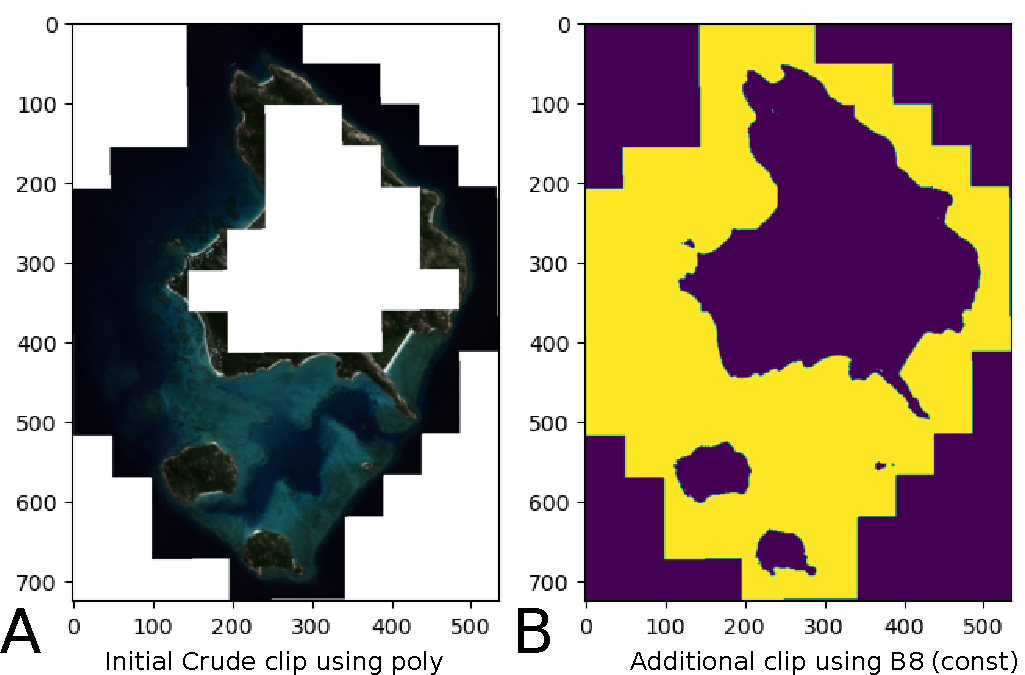
\includegraphics[width=0.7\linewidth]{Images/Preproc_Workflow.pdf}
	\caption{Clipping Image data with NIR mask, (\textbf{A}) showing original clipped Image in dataset (\textbf{B}) showing clip mask with specified threshold}
	\label{fig:PreprocWorkflow}
\end{figure}

\subsection*{color correction and color spaces}
Several methods for color correction and spaces were tested, including the use of the RGB color space, the LAB color space and the HSV color space. 
The RGB color space was chosen as the bands 4,3,2 (centered at 664, 559 and 492 nm) roughly represent the RGB color space and are most likely to penetrate the water.

We use the RGB color space as a starting point for our color correction. We then use the following color spaces to create additional features for the data, from the color spaces examined tests were run on the LAB \cite{wyszecki2000color}, HSV and HSI \cite{gonzalezr2006digital} 
color spaces respectively. This was done to preserve the overall color scheme and ensure the images are stretched correctly.  
\begin{figure}
	\centering
	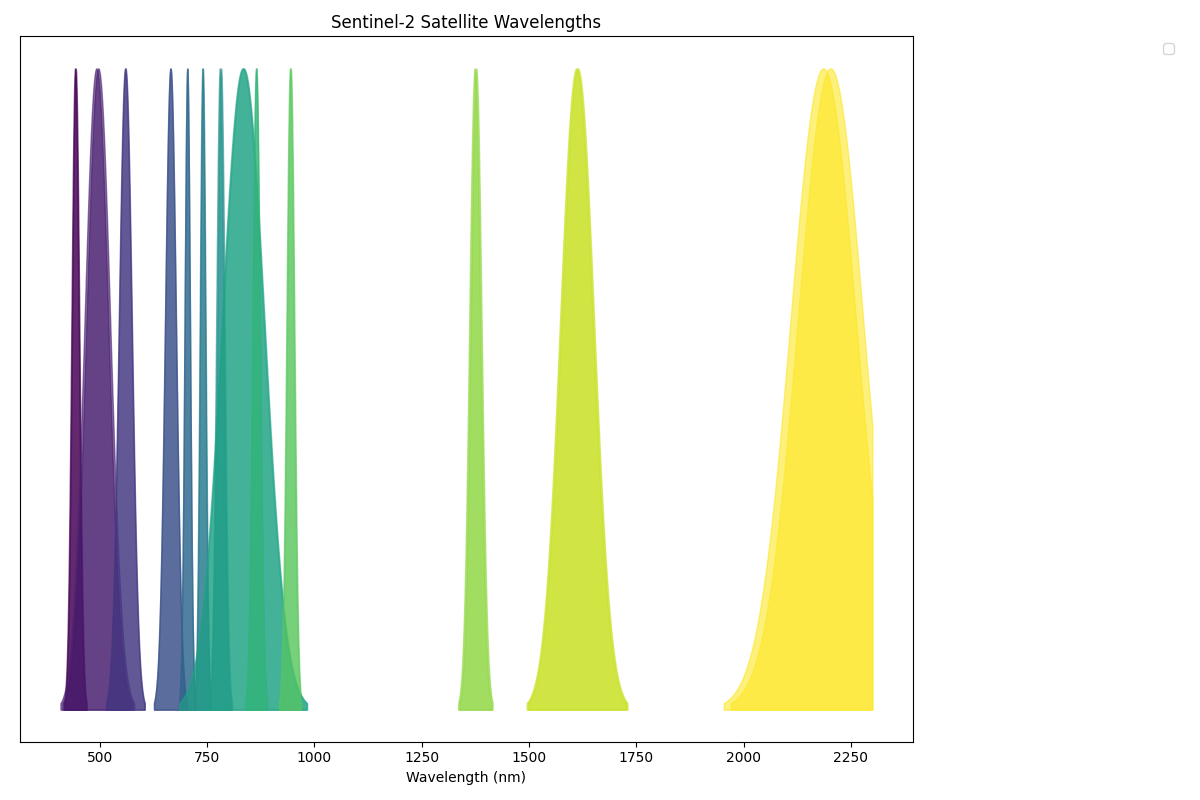
\includegraphics[width=0.7\linewidth]{Images/Sentinel-2 Wavelengths.png}
	\caption{Figure showing the wavelengths and centers of the sentinel-2A and 2B satellites}
	\label{fig:wavelengths_sen2}
\end{figure}
The images were then stacked into time series for the lizard island location, and feature generation for each individual time slice was done using the following indices:
 \begin{itemize}
	\item Chlorophyll Index (CI): Used to estimate chlorophyll content in vegetation. This information can give insights into the health and vigor of plants.
	
	\item Ocean color Index (OCI): Used to assess ocean color properties, particularly the presence of chlorophyll. This index can help in studying phytoplankton abundance and water quality in marine environments.
	
	\item Suspended Sediment Index (SSI): Used to estimate the concentration of suspended sediments in water bodies. This index is helpful in monitoring water quality, sediment transport, and erosion processes.
	
	\item Turbidity Index (TI): Used to estimate the turbidity in water bodies. Like the SSI, this index is also useful in monitoring water quality, sediment transport, and erosion processes.
	
	\item Water Quality Index (WQI): Used to assess water quality based on multiple parameters. It provides a comprehensive measure of water health, considering the contributions of various spectral bands to the index computation.
	
	\item Normalized Difference Chlorophyll Index (NDCI): Used to estimate chlorophyll content in vegetation. The NDCI provides a normalized measure of the difference between green reflectance and red-edge reflectance, indicating vegetation health.
	
	\item Blue to Green Ratio (BGR): Used to assess water quality by comparing the blue and green reflectance values. This index provides information about the concentration of chlorophyll and suspended sediments in water bodies.
	
	\item In addition to these indices, the code contains a function for masking out land areas in an image (\texttt{mask\_land}) using the NIR band and threshold, generally named the black pixel approximation \cite{siegel2000atmospheric}.
\end{itemize}
Resulting in a total of approximately ~1 million unique data points covering the range of the time series containing the original 13 bands and 7 additional features.



\subsection*{Unsupervised learning}
These are then entered into 3 dimensionality reduction algorithms, PCA \cite{pearson1901}, t-SNE \cite{van2008visualizing} and UMAP \cite{mcinnes2018umap}. These dimensionality reduction algorithms are then used to reduce the dimensionality of the data to 2 dimensions. These are then used to cluster the data using a combination of K-means, DBSCAN and HDBSCAN. The clusters retrieved from these algorithms 
are then visualised and analysed to create psuedo-labels using k-means \cite{macqueen1967some} and gaussian mixture models were also tested \cite{rasmussen1999infinite}. After hyper parameter tuning and optimisation, we then use these as labels for the supervised learning algorithm classifier which provides
additional scope for creating probability maps and testing the accuracy of the clusters themselves. 




% \begin{quote}
% This is an example of a quote.
% \end{quote}

%%%%%%%%%%%%%%%%%%%%%%%%%%%%%%%%%%%%%%%%%%
\section{Results}

\subsection*{Clustering Results}
We find that 10 clusters is the optimal number of clusters for the Lizard Island dataset, this is based on the silhouette score and the visual inspection of the clusters. This is based on several visualisations of the clusters, including the t-SNE and UMAP visualisations. 
The clusters are also tested using a combination of K-means, DBSCAN and HDBSCAN. The results of the clustering are shown in Figure \ref{fig:ClusteringResults - placeholder}. These clusters align fairly well with published work from \citep{Kennedy2021}. 

We also find that optimizing the algorithm per individual time-step also provides more consistent results for extracting the relavent reef information, using the previous clusters
centers we are able to get repeatable clusters for all of the time series, which allows for a rough approximation of what is occuring throughout the time series.

We generally find that the imagery is not always easily comparable through time, even using ratioing techniques we do not find clear repeatable clusters. This is likely due to the fact that the imagery is not always radiometrically normalised correctly, to combat this, 
performing a histogram normalisation on the data before clustering, along the entire time series itself with with reference to an initial source image, we find that the clusters become much more consistent
through time.  



\subsection*{Alternative color spaces}
By manipulating the data into various color spaces, we are able to effectively overcome some of the issues related with the original data being improperly stretched, allowing the original clustering workflow to work more effectively on various time slices that may not be radiometrically
normalised correctly, whilst this process does not adhere properly to conventional remote sensing workflows, we show that the output imagery is generally improved upon qualitative visual inspection but as the values
themselves are shifted this approach proves to actually degrade the performance of the algorithm. 

\section{Discussion}
Authors should discuss the results and how they can be interpreted from the perspective of previous studies and of the working hypotheses. The findings and their implications should be discussed in the broadest context possible. Future research directions may also be highlighted.
\begin{figure}
	\centering
	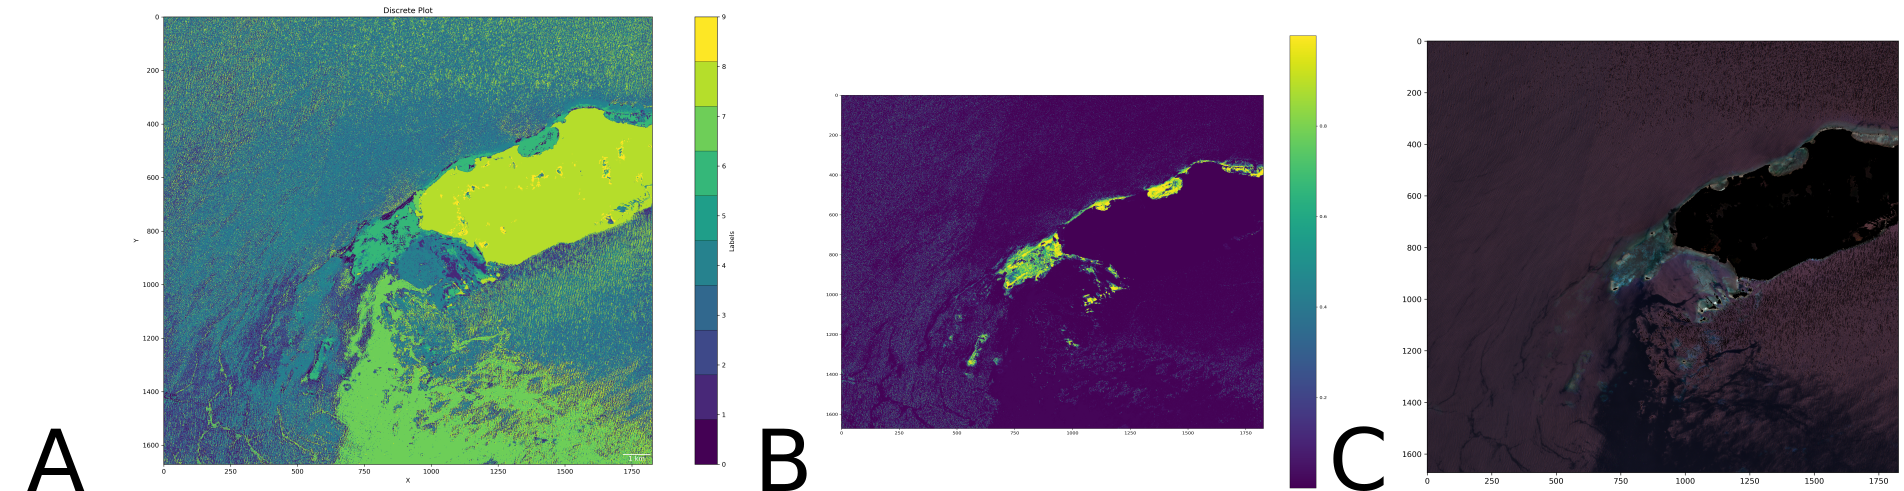
\includegraphics[width=0.7\linewidth]{Images/Honduras_Prediction.png}
	\caption{\bf{A} Overall prediction using a gradient boosting algorithm trained on the 10 original unsupervised clusters on Lizard Island, prediction is on a scene from Honduras. \bf{B} Individual class probability map generated using the same algorithm for the reef class, colorbar shows the probability of each individual pixel belonging to the reef class.
	\bf{C} Original image of the scene from Honduras.}
	\label{fig:UnsupervisedWorkflow}
\end{figure}
In this study we show that it is possible to achieve repeatable results using a combination of unsupervised and supervised learning methods to classify shallow water imagery in Sentinel-2 imagery. 
We also show that it is possible to use these methods to create a probability map of a variety of shallow water classes (will expand this) with minimal preprocessing to cluster various times in different scenes and that this methodology can be applied to different geographies whilst 
using simple explainable algorithms. 

%%%%%%%%%%%%%%%%%%%%%%%%%%%%%%%%%%%%%%%%%%
\section{Conclusions}

The research presented demonstrates an efficient and quick approach to habitat mapping, underlining the importance of the use of high-resolution satellite imagery. The results show that the proposed approach is able to provide a good classification of the habitats, with an overall accuracy of 80\%. The results are comparable to those obtained by other authors using different approaches. The proposed approach is also able to provide a good classification of the habitats, with an overall accuracy of 70 to 80\% using simple regression methods. 
The results are comparable to those published in other machine learning studies whilst remaining explainable, we also show that a workflow reliant on pixel-based methods remains viable.

Future research could benefit from incorporating specific local spectral indices in order to be more generalisable to other areas. The use of a larger training set and or ground truthed labelled data would also be benificial as this would allow more accurate validation of the results. 

Our research shows that a simple approach for pixel classification and clustering is viable for large scale monitoring of coral reefs across a wide range of geographical and ecological contexts, and that the use of sentinel-2 satellite imagery is a viable companion to more expensive methods.
%%%%%%%%%%%%%%%%%%%%%%%%%%%%%%%%%%%%%%%%%%


%%%%%%%%%%%%%%%%%%%%%%%%%%%%%%%%%%%%%%%%%%
\vspace{6pt} 

%%%%%%%%%%%%%%%%%%%%%%%%%%%%%%%%%%%%%%%%%%
%% optional
%\supplementary{The following supporting information can be downloaded at:  \linksupplementary{s1}, Figure S1: title; Table S1: title; Video S1: title.}

% Only for journal Methods and Protocols:
% If you wish to submit a video article, please do so with any other supplementary material.
% \supplementary{The following supporting information can be downloaded at: \linksupplementary{s1}, Figure S1: title; Table S1: title; Video S1: title. A supporting video article is available at doi: link.}

% Only for journal Hardware:
% If you wish to submit a video article, please do so with any other supplementary material.
% \supplementary{The following supporting information can be downloaded at: \linksupplementary{s1}, Figure S1: title; Table S1: title; Video S1: title.\vspace{6pt}\\
%\begin{tabularx}{\textwidth}{lll}
%\toprule
%\textbf{Name} & \textbf{Type} & \textbf{Description} \\
%\midrule
%S1 & Python script (.py) & Script of python source code used in XX \\
%S2 & Text (.txt) & Script of modelling code used to make Figure X \\
%S3 & Text (.txt) & Raw data from experiment X \\
%S4 & Video (.mp4) & Video demonstrating the hardware in use \\
%... & ... & ... \\
%\bottomrule
%\end{tabularx}
%}

%%%%%%%%%%%%%%%%%%%%%%%%%%%%%%%%%%%%%%%%%%
\authorcontributions{For research articles with several authors, a short paragraph specifying their individual contributions must be provided. The following statements should be used ``Conceptualization, X.X. and Y.Y.; methodology, X.X.; software, X.X.; validation, X.X., Y.Y. and Z.Z.; formal analysis, X.X.; investigation, X.X.; resources, X.X.; data curation, X.X.; writing---original draft preparation, X.X.; writing---review and editing, X.X.; visualization, X.X.; supervision, X.X.; project administration, X.X.; funding acquisition, Y.Y. All authors have read and agreed to the published version of the manuscript.'', please turn to the  \href{http://img.mdpi.org/data/contributor-role-instruction.pdf}{CRediT taxonomy} for the term explanation. Authorship must be limited to those who have contributed substantially to the work~reported.}

\funding{Please add: ``This research received no external funding'' or ``This research was funded by NAME OF FUNDER grant number XXX.'' and  and ``The APC was funded by XXX''. Check carefully that the details given are accurate and use the standard spelling of funding agency names at \url{https://search.crossref.org/funding}, any errors may affect your future funding.}

\institutionalreview{In this section, you should add the Institutional Review Board Statement and approval number, if relevant to your study. You might choose to exclude this statement if the study did not require ethical approval. Please note that the Editorial Office might ask you for further information. Please add “The study was conducted in accordance with the Declaration of Helsinki, and approved by the Institutional Review Board (or Ethics Committee) of NAME OF INSTITUTE (protocol code XXX and date of approval).” for studies involving humans. OR “The animal study protocol was approved by the Institutional Review Board (or Ethics Committee) of NAME OF INSTITUTE (protocol code XXX and date of approval).” for studies involving animals. OR “Ethical review and approval were waived for this study due to REASON (please provide a detailed justification).” OR “Not applicable” for studies not involving humans or animals.}

\informedconsent{Any research article describing a study involving humans should contain this statement. Please add ``Informed consent was obtained from all subjects involved in the study.'' OR ``Patient consent was waived due to REASON (please provide a detailed justification).'' OR ``Not applicable'' for studies not involving humans. You might also choose to exclude this statement if the study did not involve humans.

Written informed consent for publication must be obtained from participating patients who can be identified (including by the patients themselves). Please state ``Written informed consent has been obtained from the patient(s) to publish this paper'' if applicable.}

\dataavailability{We encourage all authors of articles published in MDPI journals to share their research data. In this section, please provide details regarding where data supporting reported results can be found, including links to publicly archived datasets analyzed or generated during the study. Where no new data were created, or where data is unavailable due to privacy or ethical restrictions, a statement is still required. Suggested Data Availability Statements are available in section ``MDPI Research Data Policies'' at \url{https://www.mdpi.com/ethics}.} 

% Only for journal Nursing Reports
%\publicinvolvement{Please describe how the public (patients, consumers, carers) were involved in the research. Consider reporting against the GRIPP2 (Guidance for Reporting Involvement of Patients and the Public) checklist. If the public were not involved in any aspect of the research add: ``No public involvement in any aspect of this research''.}

% Only for journal Nursing Reports
%\guidelinesstandards{Please add a statement indicating which reporting guideline was used when drafting the report. For example, ``This manuscript was drafted against the XXX (the full name of reporting guidelines and citation) for XXX (type of research) research''. A complete list of reporting guidelines can be accessed via the equator network: \url{https://www.equator-network.org/}.}

\acknowledgments{In this section you can acknowledge any support given which is not covered by the author contribution or funding sections. This may include administrative and technical support, or donations in kind (e.g., materials used for experiments).}

\conflictsofinterest{Declare conflicts of interest or state ``The authors declare no conflict of interest.'' Authors must identify and declare any personal circumstances or interest that may be perceived as inappropriately influencing the representation or interpretation of reported research results. Any role of the funders in the design of the study; in the collection, analyses or interpretation of data; in the writing of the manuscript; or in the decision to publish the results must be declared in this section. If there is no role, please state ``The funders had no role in the design of the study; in the collection, analyses, or interpretation of data; in the writing of the manuscript; or in the decision to publish the results''.} 

%%%%%%%%%%%%%%%%%%%%%%%%%%%%%%%%%%%%%%%%%%
%% Optional
\sampleavailability{Samples of the compounds ... are available from the authors.}

%% Only for journal Encyclopedia
%\entrylink{The Link to this entry published on the encyclopedia platform.}

\abbreviations{Abbreviations}{
The following abbreviations are used in this manuscript:\\

\noindent 
\begin{tabular}{@{}ll}
MDPI & Multidisciplinary Digital Publishing Institute\\
DOAJ & Directory of open access journals\\
TLA & Three letter acronym\\
LD & Linear dichroism
\end{tabular}
}

%%%%%%%%%%%%%%%%%%%%%%%%%%%%%%%%%%%%%%%%%%
%% Optional
\appendixtitles{no} % Leave argument "no" if all appendix headings stay EMPTY (then no dot is printed after "Appendix A"). If the appendix sections contain a heading then change the argument to "yes".
\appendixstart
\appendix
\section[\appendixname~\thesection]{}
\subsection[\appendixname~\thesubsection]{}
The appendix is an optional section that can contain details and data supplemental to the main text---for example, explanations of experimental details that would disrupt the flow of the main text but nonetheless remain crucial to understanding and reproducing the research shown; figures of replicates for experiments of which representative data are shown in the main text can be added here if brief, or as Supplementary Data. Mathematical proofs of results not central to the paper can be added as an appendix.

\begin{table}[H] 
\caption{This is a table caption.\label{tab5}}
\newcolumntype{C}{>{\centering\arraybackslash}X}
\begin{tabularx}{\textwidth}{CCC}
\toprule
\textbf{Title 1}	& \textbf{Title 2}	& \textbf{Title 3}\\
\midrule
Entry 1		& Data			& Data\\
Entry 2		& Data			& Data\\
\bottomrule
\end{tabularx}
\end{table}

\section[\appendixname~\thesection]{}
All appendix sections must be cited in the main text. In the appendices, Figures, Tables, etc. should be labeled, starting with ``A''---e.g., Figure A1, Figure A2, etc.

%%%%%%%%%%%%%%%%%%%%%%%%%%%%%%%%%%%%%%%%%%
\begin{adjustwidth}{-\extralength}{0cm}
%\printendnotes[custom] % Un-comment to print a list of endnotes

\reftitle{References}

% Please provide either the correct journal abbreviation (e.g. according to the “List of Title Word Abbreviations” http://www.issn.org/services/online-services/access-to-the-ltwa/) or the full name of the journal.
% Citations and References in Supplementary files are permitted provided that they also appear in the reference list here. 

%=====================================
% References, variant A: external bibliography
%=====================================
\bibliographystyle{plainnat}
\bibliography{export}

% If authors have biography, please use the format below
%\section*{Short Biography of Authors}
%\bio
%{\raisebox{-0.35cm}{\includegraphics[width=3.5cm,height=5.3cm,clip,keepaspectratio]{Definitions/author1.pdf}}}
%{\textbf{Firstname Lastname} Biography of first author}
%
%\bio
%{\raisebox{-0.35cm}{\includegraphics[width=3.5cm,height=5.3cm,clip,keepaspectratio]{Definitions/author2.jpg}}}
%{\textbf{Firstname Lastname} Biography of second author}

% For the MDPI journals use author-date citation, please follow the formatting guidelines on http://www.mdpi.com/authors/references
% To cite two works by the same author: \citeauthor{ref-journal-1a} (\citeyear{ref-journal-1a}, \citeyear{ref-journal-1b}). This produces: Whittaker (1967, 1975)
% To cite two works by the same author with specific pages: \citeauthor{ref-journal-3a} (\citeyear{ref-journal-3a}, p. 328; \citeyear{ref-journal-3b}, p.475). This produces: Wong (1999, p. 328; 2000, p. 475)

%%%%%%%%%%%%%%%%%%%%%%%%%%%%%%%%%%%%%%%%%%
%% for journal Sci
%\reviewreports{\\
%Reviewer 1 comments and authors’ response\\
%Reviewer 2 comments and authors’ response\\
%Reviewer 3 comments and authors’ response
%}
%%%%%%%%%%%%%%%%%%%%%%%%%%%%%%%%%%%%%%%%%%
\PublishersNote{}
\end{adjustwidth}
\end{document}

